\section{Results and Discussion}

\begin{figure}[!ht]
    \centering
    \raggedright
    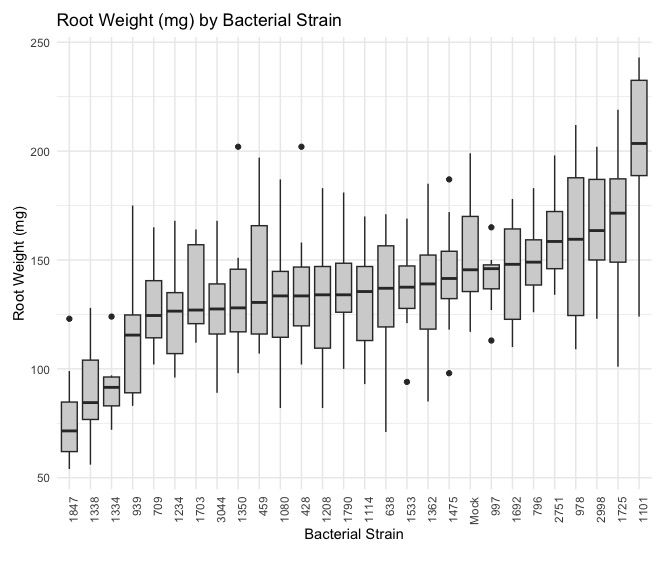
\includegraphics[width=\linewidth]{Figures/Root Weight.jpeg}
    \caption{Root weight of barley after bacterial treatment.}
    \medskip
    \textbf{Description:} The boxplot shows the distribution of root weight (in mg) for barley plants treated with different bacterial strains, sorted by the median root weight.
    \label{fig:root_length_boxplot}
\end{figure}% Root Length Boxplot

\begin{figure}[!ht]
    \centering
    \raggedright
    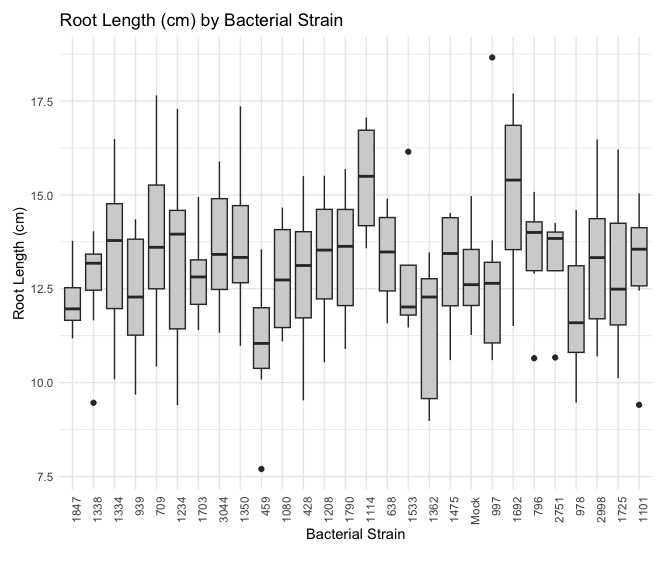
\includegraphics[width=\linewidth]{Figures/RootLength.jpeg}
    \caption{Root length of barley after bacterial treatment.}
    \medskip
    \textbf{Description:} The boxplot shows the distribution of root lengths (in cm) for barley plants treated with different bacterial strains, sorted by the median root weight.
    \label{fig:root_length_boxplot}
\end{figure}

% Heatmap
\begin{figure}[!ht]
    \centering
    \raggedright
    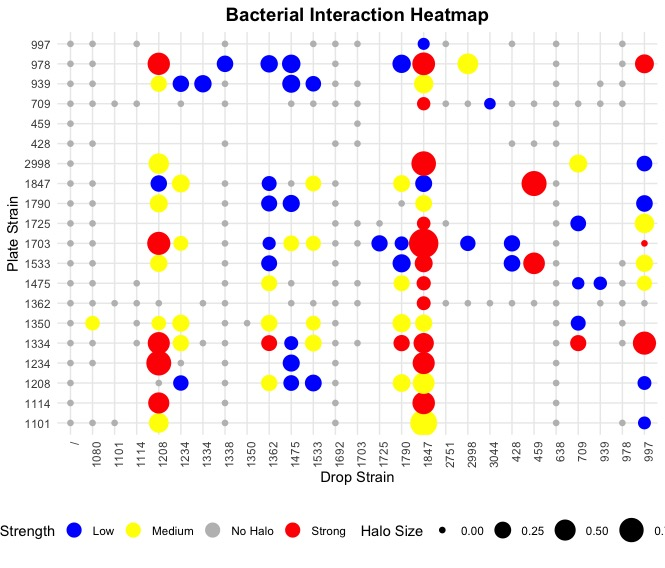
\includegraphics[width=\linewidth]{Figures/Heatmap.jpeg}
    \caption{Bacterial interaction heatmap}
    \medskip
    \textbf{Description:} The heatmap visualizes the interactions between bacterial strains, with halo size and strength indicating antagonistic effects. Grey dots represent no observed halo while the absence of a dot indicated no bacterial growth.
    \label{fig:heatmap}
\end{figure}
\begin{figure}[!ht]
    \centering
    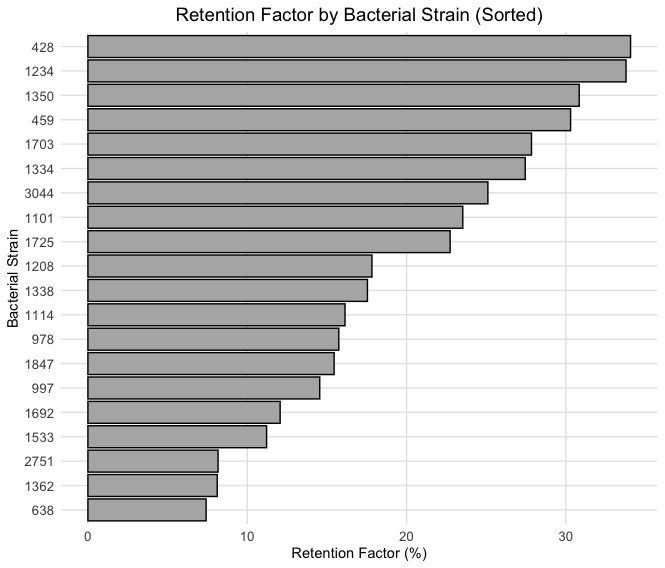
\includegraphics[width=\linewidth]{Figures/RetentionFactor.jpeg}
    \caption{Retention Factor by Bacterial Strain.}
    The retention factor measures the degree of inhibition caused by bacterial strains. 
    See the text below for details on the calculation.
    \label{fig:retention}
\end{figure}

\vspace{0.5cm} % Add space between the figure and the detailed explanation

\noindent
The retention factor is calculated using the formula:
\[
\text{Inhibition (\%)} = \frac{\text{Control Distance} - \text{Bacteria Distance}}{\text{Control Distance}} \times 100
\]
where the \textit{Control Distance} refers to the growth measurement in the absence of bacterial interference, and the \textit{Bacteria Distance} refers to the growth measurement in the presence of bacterial strains. Higher retention factor values indicate greater inhibition by the bacterial strain. The bar plot in \autoref{fig:retention} visualizes the retention factors for each bacterial strain, highlighting differences in inhibitory effects across strains.